\documentclass[border=0pt, 12pt, tikz]{standalone}
\usepackage{pgfplots}

\newcommand\Min{0}
\newcommand\Max{350}
% \pgfplotsset{domain = \Min : \Max}


\begin{document}
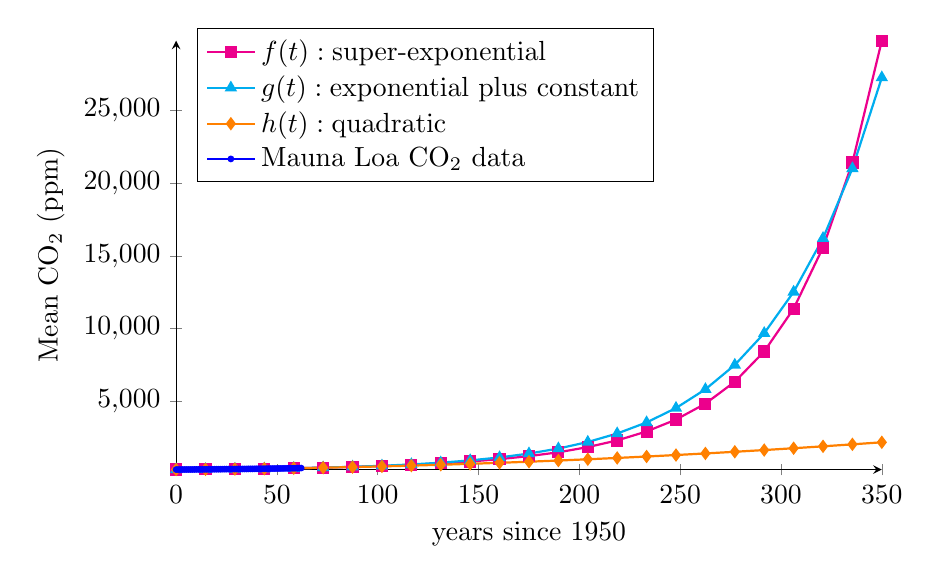
\begin{tikzpicture} 
\begin{axis}%   
[ axis lines = left
, width=300pt
, height=200pt
% , ymode = log
, xlabel = {years since 1950}
, ylabel = {Mean CO$_2$ (ppm)}     
% , y label style = {yshift = 1em}
, ylabel near ticks  % fixes position of ylabel (so that it does not crash with ticks)
, scaled ticks=false % removes scaling on axis
, yticklabel style={/pgf/number format/fixed} %avoids scientific notation on axis
% , ymax=420
% , ymin=300
% , xmax = 65
% , xmin = 0
% , log ticks with fixed point
% , grid = both
% , ytick ={300,320, 340, ...,420}
, legend style = {at={(0.03,0.85)},anchor=west} % The command for legend position
, legend cell align = {left} % The command for legend alignment
] 

% Model 1 - super exponential
\addplot%
[ color = magenta
% , only marks
, mark = square*
, mark options = {scale = 0.9}
, style = thick
, domain = \Min:\Max
]%
{315.98*(1.0026+0.00003*x)^x};%
% node[above left,pos=0.7]{$f(t)=315.98(1.0026+0.00003t)^t$}; 
\addlegendentry{$f(t): \mbox{super-exponential}$};

% Model 2 -  exponential plus constant
\addplot%
[ color = cyan
, domain = \Min:\Max
, style = thick
, mark = triangle*
, mark options = {scale = 0.9}
]%
{267.277+48.703*(1.01823)^x};%
% node[below right,pos=0.3]{$g(t)=267.277+48.703(1.01823)^t$};
\addlegendentry{$g(t): \mbox{exponential plus constant}$};

% Model 3 - quadratic
\addplot%
[ color = orange
, domain = \Min:\Max
, style = thick
, mark = diamond*
, mark options = {scale = 0.9}
]%
{0.013*x^2+0.8055*x+315.5219};%
% node[below right,pos=0.3]{$g(t)=267.277+48.703(1.01823)^t$};
\addlegendentry{$h(t): \mbox{quadratic}$};

% C02 data
\addplot%
[ color = blue
% , only marks
, mark = *
, mark options = {scale = 0.4}
, style = thick
% , mark=none
] coordinates {%
(0,  315.98)
(1,  316.91)
(2,  317.64)
(3,  318.45)
(4,  318.99)
(5,  319.62)
(6,  320.04)
(7,  321.37)
(8,  322.18)
(9,  323.05)
(10, 324.62)
(11, 325.68)
(12, 326.32)
(13, 327.46)
(14, 329.68)
(15, 330.19)
(16, 331.12)
(17, 332.03)
(18, 333.84)
(19, 335.41)
(20, 336.84)
(21, 338.76)
(22, 340.12)
(23, 341.48)
(24, 343.15)
(25, 344.85)
(26, 346.35)
(27, 347.61)
(28, 349.31)
(29, 351.69)
(30, 353.2)
(31, 354.45)
(32, 355.7)
(33, 356.54)
(34, 357.21)
(35, 358.96)
(36, 360.97)
(37, 362.74)
(38, 363.88)
(39, 366.84)
(40, 368.54)
(41, 369.71)
(42, 371.32)
(43, 373.45)
(44, 375.98)
(45, 377.7)
(46, 379.98)
(47, 382.09)
(48, 384.02)
(49, 385.83)
(50, 387.64)
(51, 390.1)
(52, 391.85)
(53, 394.06)
(54, 396.74)
(55, 398.87)
(56, 401.01)
(57, 404.41)
(58, 406.76)
(59, 408.72)
(60, 411.66)
(61, 414.24)
(62, 416.45)
};
\addlegendentry{Mauna Loa CO$_2$ data};

\end{axis} 
\end{tikzpicture}
\end{document}